\chapter{実装}
\label{chapter:proposal}

\section{減算型表示のプロトタイプ}
  \begin{figure}[t]
    \begin{center}
    \begin{minipage}{0.3\hsize}
        \begin{center}
            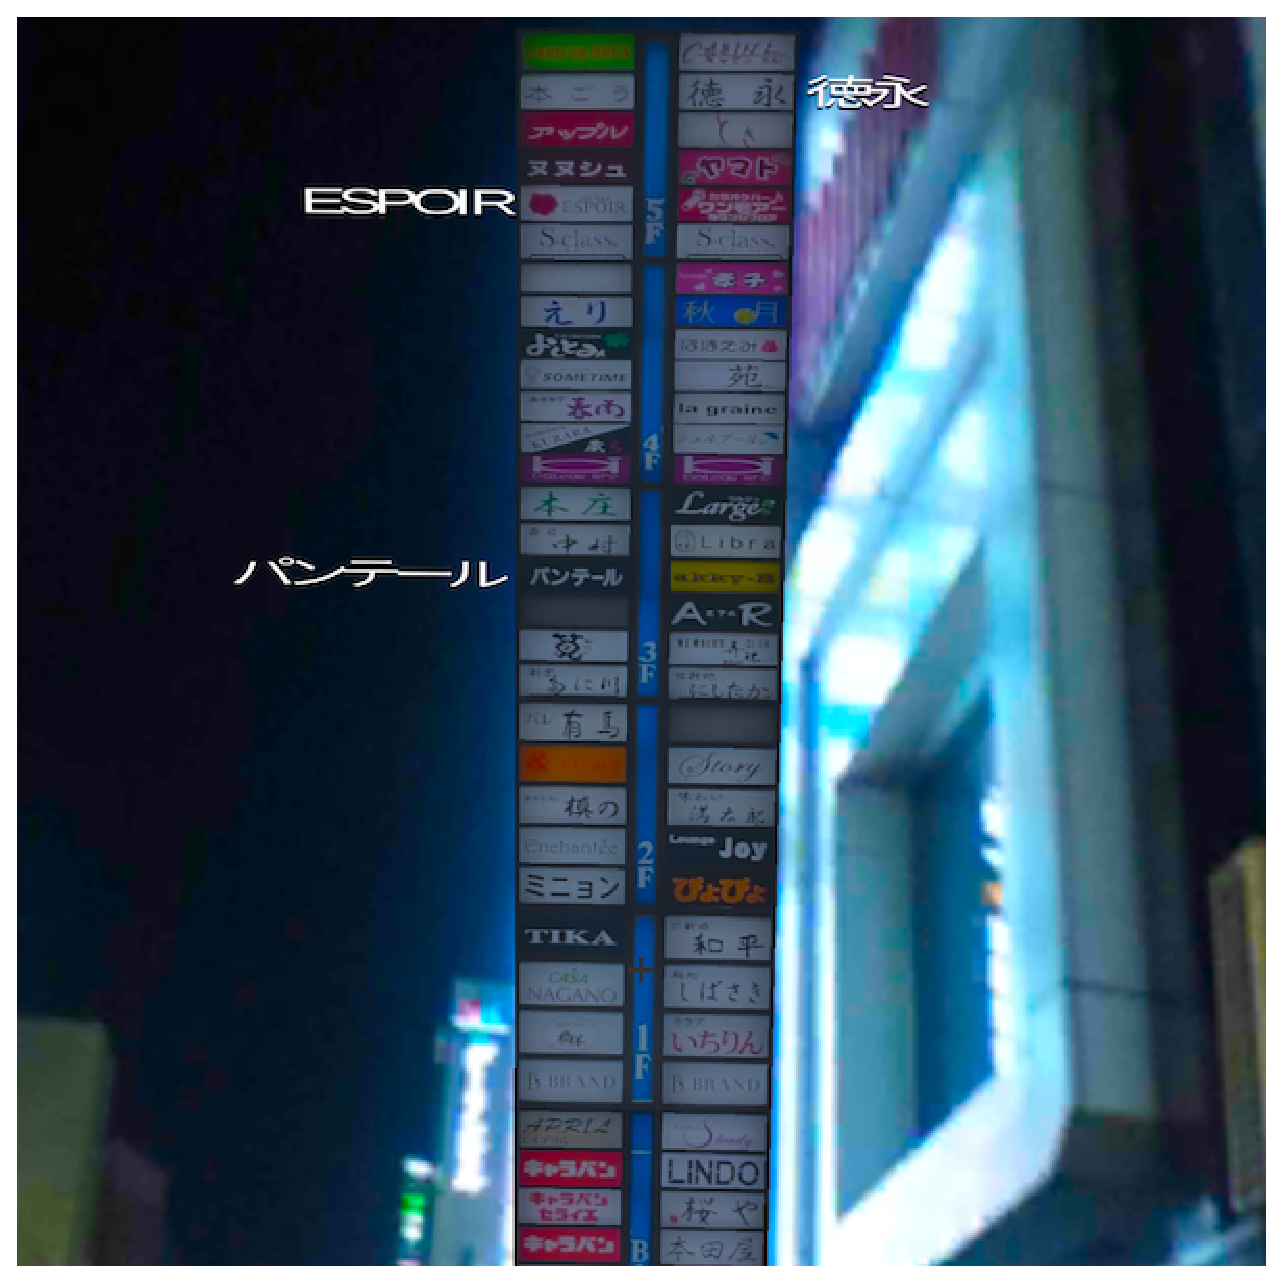
\includegraphics[clip, width=.95\textwidth]{dr_method1.eps}\\
            \small{(a) 加算型}
        \end{center}
    \end{minipage}
    \begin{minipage}{0.3\hsize}
        \begin{center}
            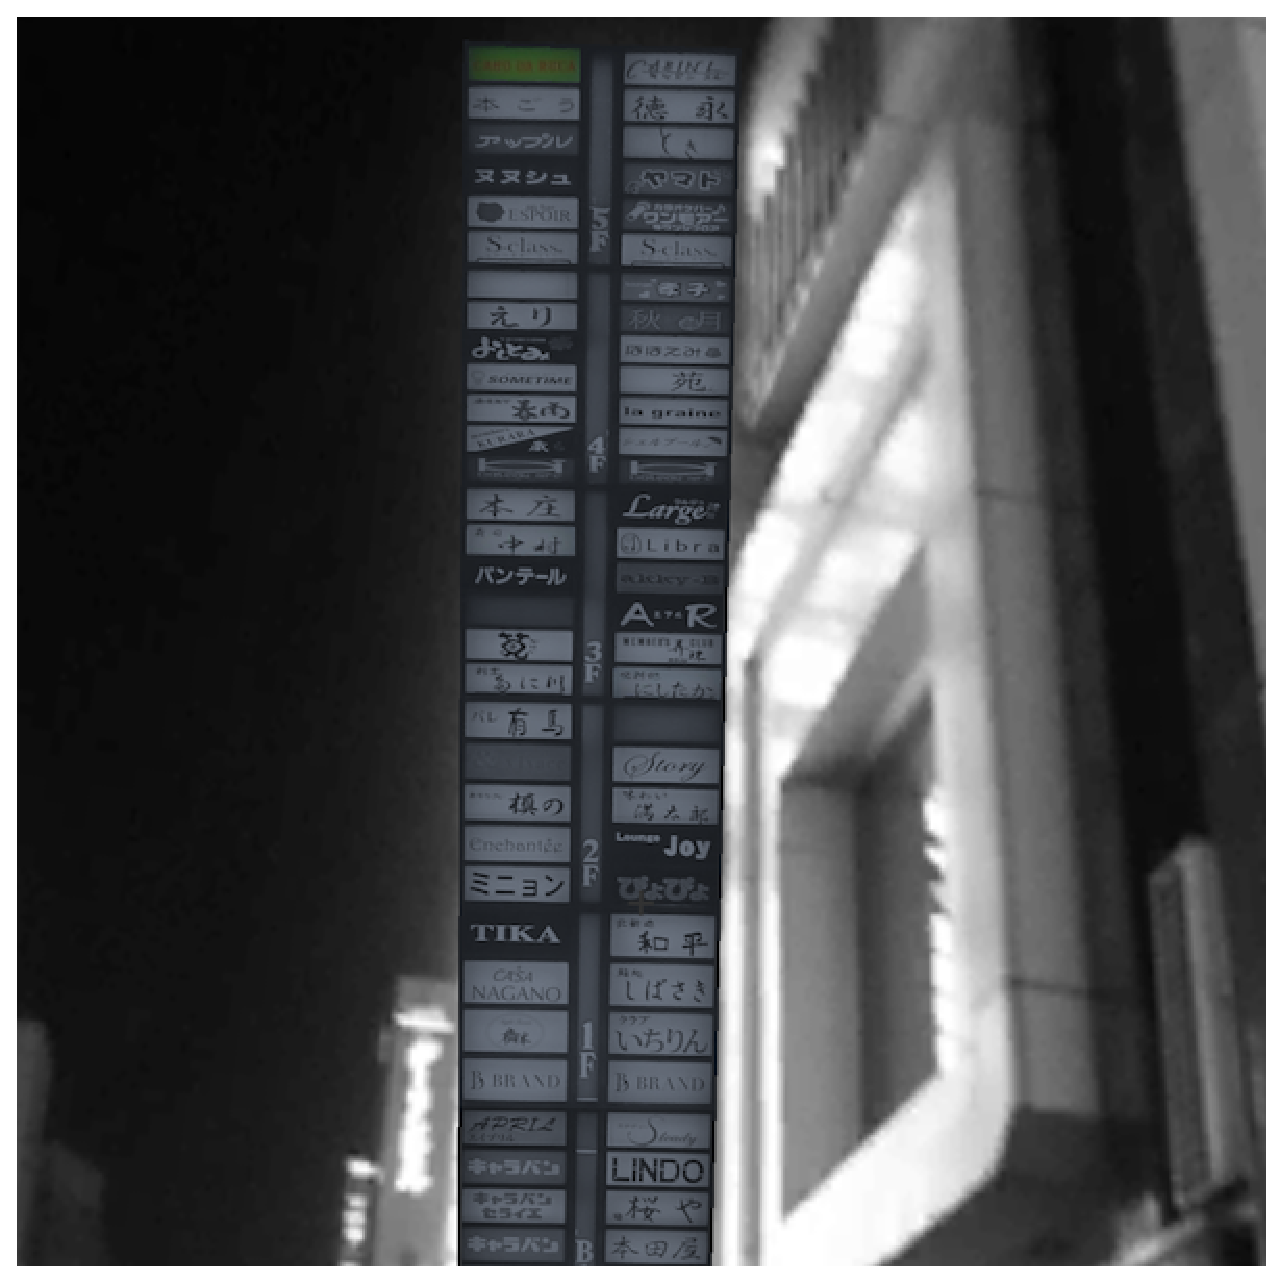
\includegraphics[clip, width=.95\textwidth]{dr_method2.eps}\\
            \small{(b) 減算型}
        \end{center}
    \end{minipage}
    \begin{minipage}{0.3\hsize}
        \begin{center}
            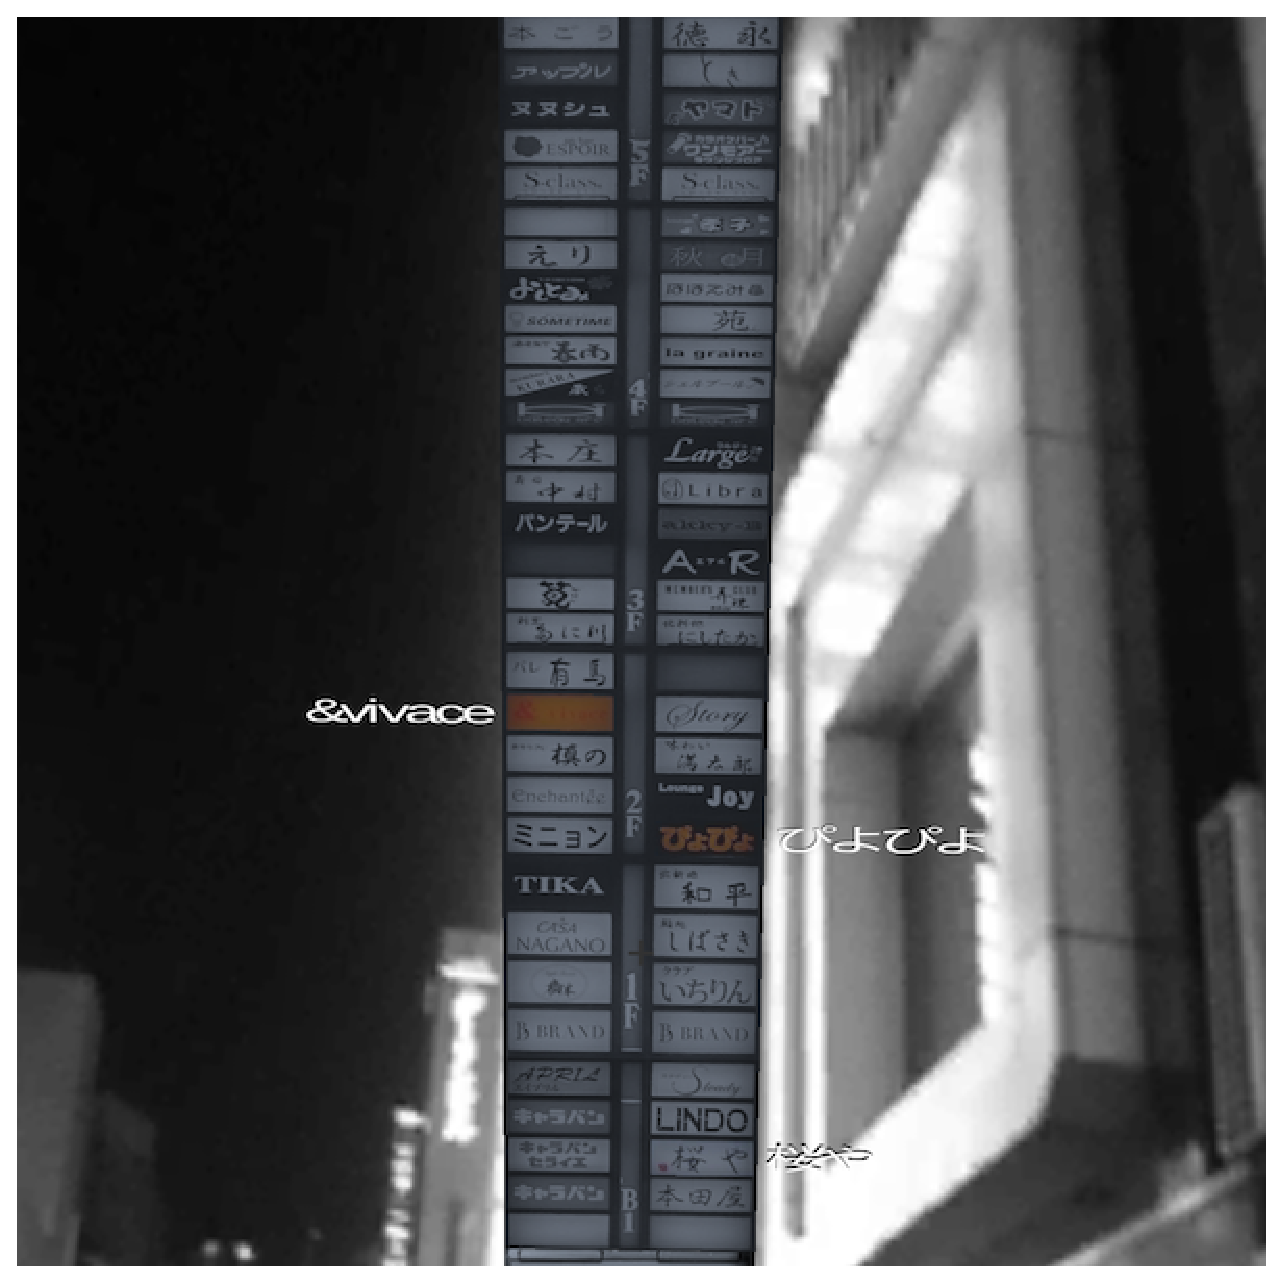
\includegraphics[clip, width=.95\textwidth]{dr_method3.eps}\\
            \small{(c) ハイブリッド型}
        \end{center}
    \end{minipage}
    \end{center}
    \vspace{1pt}
    \caption{プロトタイプの出力画面}
    \label{fig:prototype}
  \end{figure}
  本節では,?章で述べる実験に用いるプロトタイプシステムについて述べる.実験用のプロトタイプは,モバイルデバイス上で実行できるようUnity(ver 5.6.0f3)を用いてC\#言語で実装した.実環境に近づけるために,RECOH THETA\footnote{\url{https://theta360.com/}(2017/4/27確認)}を用いて新日本新地ビル付近で撮影した昼と夜の全天球画像を用意し,モバイルデバイスを通して見回せるようにした.全天球画像では看板が鮮明に撮影できないため,看板は別に撮影した画像をオブジェクトとして設置した.

  実験に用いる看板情報は,図\ref{fig:kitashinchi} - (a) に示す大阪府北新地の新日本新地ビルに掲示されている61枚の看板を用いた.店舗の種類は北新地総合情報サイト\footnote{\url{http://kgnet.jp/}(2017/4/27確認)}を参考に,「スナック・ラウンジ」,「バー」,「和食」,「居酒屋」,「クラブ」,「寿司」,「中華料理」,「ドレスショップ」の8種類に分類した.サイトに記載がなかった店舗は,「その他」として分類した.データベースはSQLite\footnote{\url{https://www.sqlite.org/}(2017/4/27確認)}(ver 3.8.10.2)を用いて,画像内の看板の位置,店舗の名前,店舗の種類,看板画像をそれぞれ格納した.

  プロトタイプでは,ユーザはモバイルデバイスを全天球画像内で全方向に向けることができる.画面中央に照準を表示し,システムは照準のローカル座標と看板のワールド座標を対応させることにより,特定の看板が選択されたことを認識できる.情報提示手法に関しては,
  \begin{itemize}
    \item 加工なし(以下,通常型と記す)
    \item 看板の横に店舗名を表示(図\ref{fig:prototype} - (a) ,以下,加算型と記す)
    \item 特定の看板以外の情報をグレースケール化(図\ref{fig:prototype} - (b) ,以下,減算型と記す)
    \item 特定の看板以外の情報をグレースケール化し,看板の横に店舗名を表示(図\ref{fig:prototype} - (c) ,以下,ハイブリッド型と記す)
  \end{itemize}
  の4種類を切り替えられるようにし,探索対象の看板は,店舗の種類別に切り替えられるようにした.また,ユーザがスタートボタンをタップしてから特定の看板を見つけるまでの所要時間を計測できる機能を用意した.ユーザが特定の看板に照準を1秒間合わせると,看板を見つけたと判定するよう実装した.

\section{リアルタイム看板認識APIの実装}

    \begin{table}[t]
    \caption{プロトタイプに用いたデータ(2018年12月時点OSMのデータベースを基に作成)}
    \label{tab:storelist}
    \begin{center}
      \begin{small}
        \begin{tabular}{c|cccccc}
        \hline\hline
        id & name & shop/amenity & opening\_hours & payment:visa \\ 
        \hline
        2391866925 & セブン-イレブン 高槻高槻町店 & convenience & 24/7 & yes \\
        5279265335 & 全席個室居酒屋 北海の恩返し 高槻店 & bar & 17:00-24:00 & yes \\
        5281672553 & 小だるま JR高槻駅前店 & bar & Mo-Th 11:30-14:00; \ldots & yes \\
        5281672555 & 肉丼専門店 高槻肉劇場 & restaurant & 11:00-23:00 & no \\
        5281672556 & おだいどこはなれ 高槻店 & bar & Mo-Th 11:30-24:00; \ldots & yes \\
        5281672557 & ビリヤード・ダーツ\&Food Bar Ozbuddy & pub & Mo-Th 14:00-26:00; \ldots & no \\
        5281672577 & 磯丸水産 高槻店 & restaurant & 24/7 & yes \\
        5281672578 & 炭焼酒場 森田家 高槻店 & restaurant & 17:00-26:00 & yes \\
        5281672579 & メサベルテ 高槻店 & bakery & Mo-Sa 07:00-20:30; \ldots & no \\
        5281672580 & 駿河屋 & hobby & 10:00-23:00 & no \\
        5281672581 & 甲南チケット 高槻本通店 & ticket & Mo-Sa 10:00-19:00; \ldots & no \\
        5281672739 & 焼肉・しゃぶしゃぶ食べ放題ぷくぷく 高槻店 & restaurant & Mo-Fr 16:30-25:00; \ldots & yes \\
        5281672740 & 赤から 高槻店 & bar & Mo-Fr 17:00-24:00; \ldots & yes \\
        5281672835 & ちどり亭 高槻店 & restaurant & 17:00-25:00 & yes \\
        5281672942 & 高槻ちゃぶちゃぶ & bar & 17:54-06:00 & yes \\
        \hline
        \end{tabular}
      \end{small}
    \end{center}
    \end{table}

    \begin{table}[tb]
        \caption{看板画像の学習と検出に用いたマシンのスペック}
        \label{tab:machine}
        \begin{center}
        \begin{tabular}{c|c}
            \hline\hline
            要素 & スペック \\
            \hline
            CPU & Intel (R) Core (TM) i7-8700K @ 3.70 GHz \\
            RAM & 16 GB \\
            GPU & NVIDIA GeForce GTX 1080 \\
            VRAM & 12 GB \\
            OS & Ubuntu 17.10 \\
            \hline
        \end{tabular}
        \end{center}
    \end{table}

    \subsection{対象とするデータ}
    \ref{sec:system}章で述べた構成に基づき,大阪府高槻市のJR高槻駅と阪急高槻市駅の間にある商店街の一部を対象としたプロトタイプを実装する.看板の認識には,少ない学習データから高い精度での認識を可能にするために,文献\cite{Kitamura2018}で提案したAPIを用いる.
    プロトタイプでは,図\ref{fig:map}の赤線部で示されている高槻本通の$100 m$区間においてOSM上にデータが存在する店舗のうち,15店舗を対象とする.
    対象とする店舗のノードを表\ref{tab:storelist}に示す.
    OSM上では,飲食店などの店舗のオブジェクトは位置を定義された単一の点であるノードとして扱われ,各オブジェクトには``OSM ID''という一意の番号が付与されている.
    各店舗の看板画像とOSM IDを紐付け,Overpass API\footnote{http://overpass-api.de}を用いて店舗情報を取得することにより,看板画像から店舗情報へのアクセスができる.
    表\ref{tab:storelist}内の``id''は各店舗のOSM IDを表しており,それぞれのノードには複数のタグが設定されている.
    ``name''は店舗の名称が代入されている.
    ``shop''タグは,店舗が販売している商品を記述するために使用される.
    飲食店の場合,施設の種類を表す``amenity''タグにバーやレストランのような店舗の種類が代入されている.
    ``opening\_hours''タグには,店舗の営業時間が代入されている.年中無休で24時間営業の場合は``24/7''が,曜日によって営業時間が異なる場合は,セミコロン区切りで複数の値が代入されている.例えば,小だるま JR高槻駅前店は,月曜日から木曜日までは11時30分から14時00分と17時から23時30分まで,金曜日,土曜日は11時30分から14時30分と17時00分から24時30分,日曜日は11時30分から23時30分が営業時間である.この場合,``opening\_hours''タグの値は
    ``Mo-Th 11:30--14:00, 17:00--23:30; Fr-Su 11:30--14:30, 17:00--24:30; Su 11:30--23:30''となる.
    支払いにクレジットカードが利用可能かどうかは,``american\_express'',``payment:diners\_club'',``payment:jcb'',``payment:master'',``payment:visa'',のタグに``yes''が代入されていれば利用可能である.表\ref{tab:storelist}には``payment:visa''タグのみを掲載している.

  \subsection{看板画像の学習}
    看板の認識は,まず写真の中から看板領域を抽出し,次に,切り出された看板がどの店舗のものなのかを識別するという2段階で行う.
    看板画像の学習は,文献\cite{Kitamura2018}と同一の条件下で行った.学習に用いたマシンのスペックを表\ref{tab:machine}に示す.
    写真の中から看板の領域を抽出するために,Tensorflow 1.0\cite{abadi2016tensorflow}で実装されたYOLOv2\cite{YOLO9000}を用いた.
    対象とする店舗の前で様々な角度から合計650枚の写真を撮影し,それぞれに人手で看板領域をアノテーションした上で,585枚を教師データ,65枚をテストデータとして学習させた.

    抽出した看板画像から店舗名を識別するためには,VGG16\cite{VGG16}を用いた.
    表\ref{tab:storelist}に記載した15店舗の看板画像を昼の時間帯に各店舗100枚ずつ,合計1,500枚の写真を収集し,1店舗につき教師データ50枚,バリデーションデータ25枚,テストデータ25枚に分類して学習させた.

    看板認識を行うAPIは,Python \footnote{https://www.python.org} 3.6.5とWeb APIフレームワークであるFalcon \footnote{https://falconframework.org} 1.4.1を用いて,を用いて学習に用いたマシンと同一のマシンに構築したサーバ上に構築した.

\section{Scan by Snapのプロトタイプ}

\begin{figure*}[t]
    \begin{center}
      \includegraphics[clip, width=1.9\columnwidth]{recog_method.eps}
      \caption{システムの動作}
      \label{fig:method}
    \end{center}
  \end{figure*}

\subsection{ユーザインタフェース}
クライアントサイドは,ユーザがOSを問わずに携帯端末で実行できるようにするために,HTML5とJavascriptを用いてWebアプリケーションとして実装した.
インタフェースはデフォルトで端末の背面カメラ画面となっており,ユーザが前面カメラと切り替えられるようになっている.
ユーザがカメラを通して店舗の看板を見ると,その店舗の店舗名,営業時間,使えるクレジットカードの種類などの情報が表示される.
表示される店舗の種類や表示する情報の種類はユーザが選択できる.
ユーザにとって不要な情報は明度を下げることによって目立たなくしている.
実装したユーザインタフェースを図\ref{fig:interface}に示す.

\subsection{システムの動作}
提案システムにおいて,ユーザが取る行動とシステムが行う処理を以下に示し,図で表したものを図\ref{fig:method}に示す.
\begin{enumerate}
    \item システムは携帯端末のGPS機能により,ユーザの位置情報を取得する
    \item ユーザは店舗の種類などのクエリを入力する
    \item システムはOverpass APIに位置情報とクエリを送信し,クエリに一致する周辺の店舗のOSM IDを取得する
    \item ユーザは携帯端末のカメラを通して街から画像情報を取得する(図\ref{fig:method}中\textcircled{\scriptsize 1})
    \item システムは画像をサーバに送信する(図\ref{fig:method}中\textcircled{\scriptsize 2})
    \item サーバはYOLOを用いて画像の中から看板領域を検出する(図\ref{fig:method}中\textcircled{\scriptsize 3})
    \item サーバは検出された看板領域を切り抜く(図\ref{fig:method}中\textcircled{\scriptsize 4})
    \item サーバはそれぞれの看板画像をVGG16を用いて店舗名でクラス分けする(図\ref{fig:method}中\textcircled{\scriptsize 5})
    \item サーバは画像内の看板の左上と右下の座標と検出した看板の店舗と関連付けられたOSMのノードのidをそれぞれ格納したJSONデータを生成する(図\ref{fig:method}中\textcircled{\scriptsize 6})
    \item サーバは生成されたJSONをシステムに返り値として返却する(図\ref{fig:method}中\textcircled{\scriptsize 7})
    \item システムはユーザが求めていない視覚情報の色調を低減させ,ユーザが求めている店舗の情報を看板の横に吹き出しとして重畳表示する(図\ref{fig:method}中\textcircled{\scriptsize 8})
    \item システムは認識した看板と関連付けられているOSM IDをOverpass APIに送信する(図\ref{fig:method}中\textcircled{\scriptsize 9})
    \item Overpass APIはOSM IDと一致する店舗のノードをシステムに返却する(図\ref{fig:method}中\textcircled{\scriptsize 10})
    \item システムは出力結果をユーザに提示する(図\ref{fig:method}中\textcircled{\scriptsize 11})
\end{enumerate}

デバイスが画像をAPIに送信してからサーバがJSONデータを返却するまでに要した時間は,上り1Mbps,下り1.25Mbpsの通信速度,980 $\times$ 1307の解像度で平均359msであった.
Thropeらによると,人間が画面中央のオブジェクトを認識するまでのリアクションタイムの中央値は445msであるため\cite{Thorpe:1996},十分にユーザが満足できる速度であるといえる.



\section{評価すべき項目の検討}